\chapter{Risultati} \label{chp:risultati}
In questo capitolo verranno presentati i risultati ottenuti dalle due fasi di
valutazione delle diverse versioni dei modelli separati in base ai dataset su
cui sono stati allenati: \texttt{dataset\_corr} e \texttt{dataset\_pca}. Prima
verranno presentati i risultati ottenuti dalla validazione $80/20$ con gli
iperparametri migliori ottenuti nel capitolo precedente, successivamente
verranno presentati i risultati ottenuti dalla $10$-fold cross-validation.

% Prima di esporre i risultati ottenuti, è opportuno enunciare la seguente premessa.
% Considerando la natura del contesto, mirante alla classificazione di dati medici,
% si è convenuto di regolare manualmente il valore della soglia per la predizione
% del tumore. Tale decisione è stata presa al fine di minimizzare il numero di
% falsi negativi, ossia i casi in cui il modello erroneamente predice l'assenza di
% tumore quando invece è presente.

% Per effettuare questa operazione, è stato selezionato il valore di soglia pari a
% $0.3$, al fine di ridurre il numero di falsi negativi. Questa determinazione è
% stata adottata per conferire maggior rilevanza al valore di richiamo, che valuta
% l'efficacia del modello nell'individuare i veri positivi.

I classificatori sono stati valutati calcolando la matrice di confusione,
successivamente sono state calcolate le metriche associate ad essa:
\begin{itemize}
    \item \textbf{Accuracy}: misura la frazione di esempi classificati
          correttamente.
    \item \textbf{Precision}: misura la frazione di esempi classificati come
          positivi che sono effettivamente positivi.
    \item \textbf{Recall}: misura la frazione di esempi positivi che sono stati
          classificati correttamente.
    \item \textbf{F1-score}: media armonica tra precisione e recall.
\end{itemize}
Inoltre, sono state calcolate le curve ROC per analizzare TP rate e FP rate.
Infine, per la seconda fase di validazione, dal momento che è stata effettuata
una $10$-fold cross-validation, sono state calcolate per ciascuno dei 10
modelli le metriche di Accuracy, Precision, Recall e F1-score in modo da
ottenere gli intervalli di confidenza, per analizzare la robustezza dei modelli.

% Nelle successive sezioni verranno esposti i risultati ottenuti per ciascun
% modello, confrontando i valori delle metriche di valutazione e le curve ROC
% generate. I risultati saranno suddivisi in due sezioni, una per il confronto
% sul dataset le cui feature sono state selezionate manualmente, una per il
% confronto sul dataset le cui feature sono state selezionate con PCA.
\section{Risultati dei modelli allenati su \texttt{dataset\_corr} e
  \texttt{dataset\_corr\_std}} \label{sec:risultati_corr}
Per prima cosa sono state prodotte le matrici di confusione per ciascun modello
raffigurate nella figura \ref{fig:matrice_di_confusione_per_corr}.

Le matrici di confusione evidenziano che i tre modelli presentano buoni risultati
nel compito di classificazione. In particolare, sia il modello SVM che la rete
neurale mostrano performance identiche, mentre il modello Gaussian Naive Bayes è
caratterizzato da un numero maggiore di errori. Si osserva una tendenza comune a
commettere più errori nella classificazione degli esempi negativi rispetto a
quelli positivi per tutti i modelli, indicando una possibile sovrapposizione
eccessiva (overfitting) sulla classe negativa, probabilmente attribuibile a un
leggero squilibrio non significativo tra le classi presenti nel dataset.

Risulta possibile condurre un'analisi più dettagliata dei modelli mediante il
calcolo delle metriche di Accuracy, Precision, Recall e F1-score dalle matrici
di confusione. Nella tabella \ref{tab:risultati}, vengono riportati i valori di
tali metriche ottenuti per ciascun modello, calcolati sul test set. Quest'ultimo
è composto dal $20\%$ dei dati provenienti dai dataset \texttt{dataset\_corr} e
\texttt{dataset\_corr\_std}.
\begin{table}[!ht]
    \centering
    \begin{tabular}{@{}clllll@{}}
        \toprule
        \rowcolor[HTML]{EFEFEF}
        \textbf{Modello}                                      & \textbf{Accuracy}            & \textbf{Precision}           & \textbf{Recall}              & \textbf{F1-score}            & \textbf{Tempo}              \\ \midrule
        \cellcolor[HTML]{EFEFEF}\textbf{SVM}                  & \multicolumn{1}{c}{98.10 \%} & \multicolumn{1}{c}{99.38 \%} & \multicolumn{1}{c}{96.40 \%} & \multicolumn{1}{c}{97.87 \%} & \multicolumn{1}{c}{0.216 s} \\
        \cellcolor[HTML]{EFEFEF}\textbf{Gaussian Naive Bayes} & \multicolumn{1}{c}{94.05 \%} & \multicolumn{1}{c}{98.98 \%} & \multicolumn{1}{c}{87.87 \%} & \multicolumn{1}{c}{93.01 \%} & \multicolumn{1}{c}{0.006 s} \\
        \cellcolor[HTML]{EFEFEF}\textbf{Rete neurale}         & \multicolumn{1}{c}{98.93 \%} & \multicolumn{1}{c}{98.52 \%} & \multicolumn{1}{c}{99.10 \%} & \multicolumn{1}{c}{98.81 \%} & \multicolumn{1}{c}{6.363 s} \\ \bottomrule
    \end{tabular}
    \caption{Risultati ottenuti dal modello addestrato}
    \label{tab:risultati}
\end{table}

% ! Controllo il commento 
I risultati ottenuti rivelano prestazioni superiori per i modelli basati su una
manipolazione geometrica dei dati, come la rete neurale e il Support Vector
Machine (SVM), rispetto al modello fondato su una manipolazione probabilistica,
come il Gaussian Naive Bayes.

Tale fenomeno può essere motivato considerando che una feature non rispetta
la distribuzione gaussiana, quindi dal momento che si calcola la verosimiglianza
utilizzando la formula della distribuzione normale, Gaussian Naive Bayes risulta
più sensibile alla sua assunzione. Inoltre, la rete neurale e SVM sono modelli
intrinsecamente più complessi rispetto al Gaussian Naive Bayes, consentendo loro
di catturare relazioni più intricate tra le features e la variabile target. Per
lo più ritornando al diagramma di dispersione delle features alla figura
\ref{fig:scatterplot_features}, si può notare che per le features presenti in
\texttt{dataset\_corr} si hanno leggere sovrapposizioni delle classi, questo
suggerisce che a dimensioni maggiori le classi potrebbero essere più facilmente
separabili.
\begin{figure}[!ht]
    \centering
    \begin{subfigure}{0.45\textwidth}
        \centering
        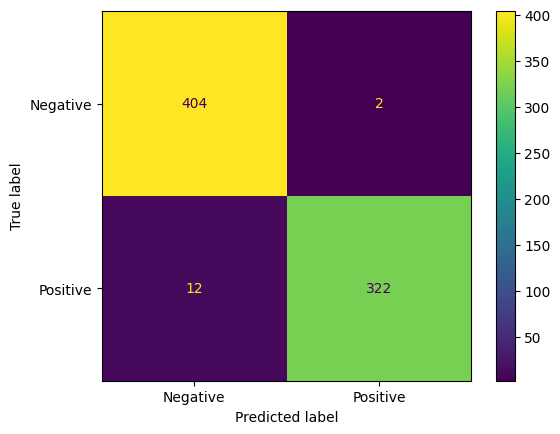
\includegraphics[width=\textwidth]{img/svm/matrice_confusione_corr.png}
        \caption{Support Vector Machine}
        \label{fig:matrice_di_confusione_per_SVM_corr}
    \end{subfigure}
    \hfill
    \begin{subfigure}{.45\textwidth}
        \centering
        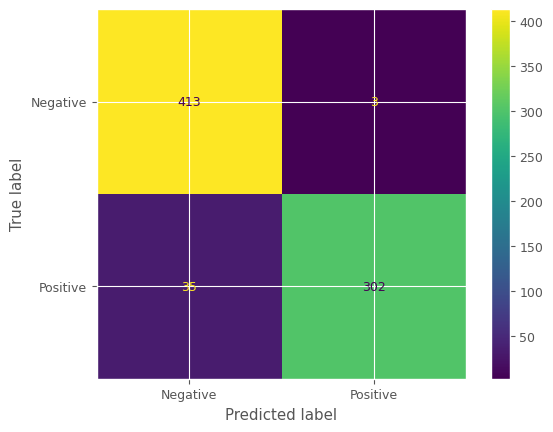
\includegraphics[width=\textwidth]{img/gnb/confusion_matrix_corr.png}
        \caption{Gaussian Naive Bayes}
        \label{fig:matrice_di_confusione_per_GNB_corr}
    \end{subfigure}
    \hfill
    \begin{subfigure}{.45\textwidth}
        \centering
        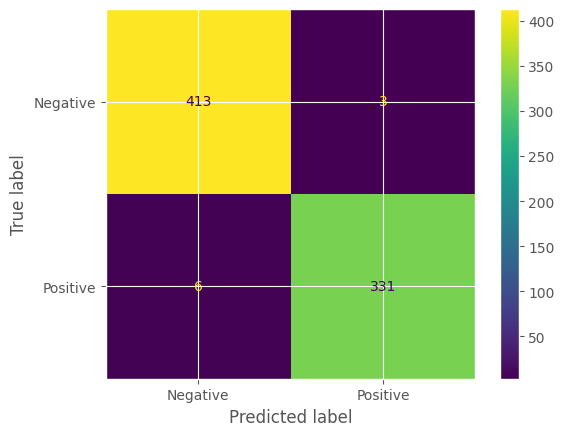
\includegraphics[width=\textwidth]{img/rete/matrice_confusione.png}
        \caption{Rete neurale}
        \label{fig:matrice_di_confusione_per_NN_corr}
    \end{subfigure}
    \caption{Matrici di confusione per i modelli addestrati su \texttt{dataset\_corr} e \texttt{dataset\_corr\_std}}
    \label{fig:matrice_di_confusione_per_corr}
\end{figure}

In seguito, si è deciso di confrontare i modelli utilizzando un ulteriore metrica,
ovvero AUC e le curve ROC, le quali permettono di confrontare i modelli in
termini di trade-off tra tasso di veri positivi e tasso di falsi positivi, in
aggiunta, le curve ROC confrontano i modelli indipendentemente dalla soglia
scelta e questo risparmia l'ottimizzazione del modello rispetto ad una
particolare soglia.

Le curve ROC del classificatore casuale e dei tre modelli allenati su
\texttt{dataset\_corr} e \texttt{dataset\_corr\_std} sono visibili nella figura
\ref{fig:roc_curve_corr}.
\begin{figure}[!ht]
    \centering
    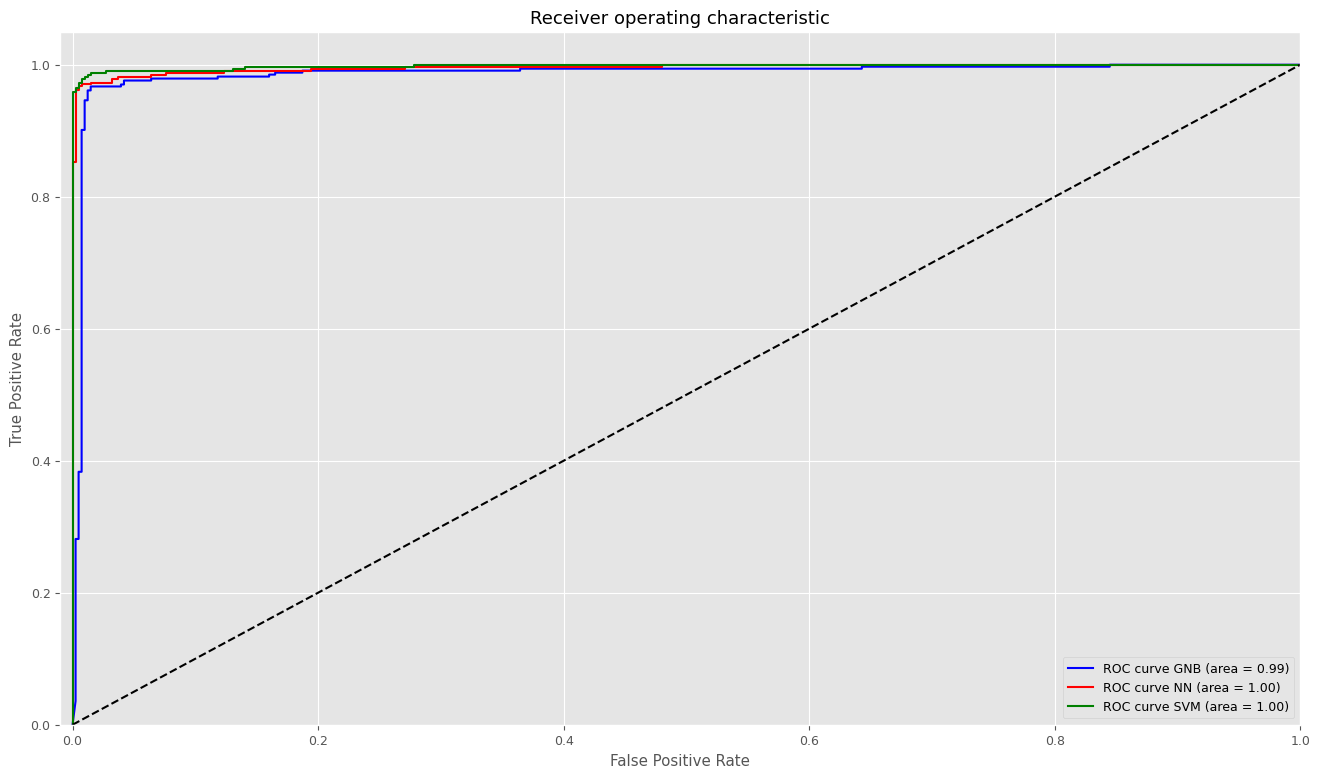
\includegraphics[width=\textwidth]{img/ris/roc_curve_corr.png}
    \caption{Curve ROC per i modelli addestrati su \texttt{dataset\_corr} e \texttt{dataset\_corr\_std}}
    \label{fig:roc_curve_corr}
\end{figure}

Il grafico riportato in figura \ref{fig:roc_curve_corr} mostra che i tre modelli
allenati hanno delle prestazioni molto simili tra loro e nettamente migliori
rispetto al classificatore randomico. Con queste premesse risulta fondamentale
concentrarsi sul confronto dell'area sottesa alla curva ROC (AUC). L'area sottesa
alla curva ROC per la rete neurale e per SVM è pari a $1.00$, mentre per il
Gaussian Naive Bayes è pari a $0.99$. Questi valori suggeriscono che i modelli
basati sulla manipolazione geometrica leggermente superiore a Gaussian Naive
Bayes in termini di capacità di discriminazione tra le due classi, anche se a
livello assoluto tutti e tre i modelli sono ottimi per la classificazione.

Come anticipato precedentemente, dal momento che il dataset è di medie
dimensioni si è deciso di effettuare anche uno studio di robustezza dei modelli.
Per fare ciò si è deciso di condurre una valutazione tramite la tecnica della
$10$-fold stratified cross-validation. Tale tecnica permette di ottenere una
stima più accurata delle performance del modello, riducendo l'effetto della
variabilità dei dati.

In questo processo ogni modello che è stato addestrato è stato valutato
attraverso le metriche di Accuracy, Precision, Recall e F1-score. I risultati
ottenuti dall'esecuzione della cross-validation sono stati utilizzati per
calcolare gli intervalli di confidenza al $90\%$ delle metriche sopracitate.

Per svolgere questa operazione sono stati utilizzati \texttt{dataset\_corr} e
\texttt{dataset\_corr\_std} completo, ovvero senza alcuna suddivisione in training
set e test set, dal momento che le separazioni vengono effettuate all'interno
della cross-validation.

I risultati ottenuti sono stati riportati sia in forma numerica che grafica
per facilitare la comprensione. In particolare, i valori delle metriche ottenuti
sono stati riportati in figura \ref{fig:img_intervalli_confidenza_corr} e
nella tabella \ref{tab:intervalli_confidenza_corr}.
\begin{table}[!ht]
    \begin{subtable}[h]{1\textwidth}
        \centering
        \begin{tabular}{@{}clllll@{}}
            \toprule
            \rowcolor[HTML]{EFEFEF}
            \textbf{Modello}                                      & \textbf{Accuracy}            & \textbf{Precision}           & \textbf{Recall}              & \textbf{F1-score}            & \textbf{Tempo}              \\ \midrule
            \cellcolor[HTML]{EFEFEF}\textbf{SVM}                  & \multicolumn{1}{c}{98.10 \%} & \multicolumn{1}{c}{99.38 \%} & \multicolumn{1}{c}{96.40 \%} & \multicolumn{1}{c}{97.87 \%} & \multicolumn{1}{c}{0.216 s} \\
            \cellcolor[HTML]{EFEFEF}\textbf{Gaussian Naive Bayes} & \multicolumn{1}{c}{94.05 \%} & \multicolumn{1}{c}{98.98 \%} & \multicolumn{1}{c}{87.87 \%} & \multicolumn{1}{c}{93.01 \%} & \multicolumn{1}{c}{0.006 s} \\
            \cellcolor[HTML]{EFEFEF}\textbf{Rete neurale}         & \multicolumn{1}{c}{98.27 \%} & \multicolumn{1}{c}{97.99 \%} & \multicolumn{1}{c}{98.15 \%} & \multicolumn{1}{c}{98.06 \%} & \multicolumn{1}{c}{6.363 s} \\ \bottomrule
        \end{tabular}
        \caption{Valore medio delle metriche ottenute dalla cross validation}
        \label{tab:risultati_cross_val_corr}
    \end{subtable}
    \hfill
    \begin{subtable}[h]{1\textwidth}
        \centering
        \begin{tabular}{@{}cllll@{}}
            \toprule
            \rowcolor[HTML]{EFEFEF}
            \textbf{Modello}                                      & \textbf{Accuracy}  & \textbf{Precision} & \textbf{Recall}    & \textbf{F1-score}  \\ \midrule
            \cellcolor[HTML]{EFEFEF}\textbf{SVM}                  & [98.71\%, 99.45\%] & [99.17\%, 99.98\%] & [97.68\%, 99.07\%] & [98.55\%, 99.39\%] \\
            \cellcolor[HTML]{EFEFEF}\textbf{Gaussian Naive Bayes} & [94.85\%, 95.84\%] & [98.76\%, 99.40\%] & [89.49\%, 91.59\%] & [94.01\%, 95.21\%] \\
            \cellcolor[HTML]{EFEFEF}\textbf{Rete neurale}         & [97.98\%, 98.55\%] & [97.47\%, 98.52\%] & [97.49\%, 98.81\%] & [97.75\%, 98.38\%] \\ \bottomrule
        \end{tabular}
        \caption{Intervalli di confidenza delle metriche ottenute dalla cross validation}
        \label{tab:intervalli_confidenza_corr}
    \end{subtable}
    \caption{Risultati ottenuti dalla cross validation}
    \label{tab:metriche_intervalli_confidenza_corr}
\end{table}
\begin{figure}[!ht]
    \centering
    \begin{subfigure}[b]{0.4\textwidth}
        \centering
        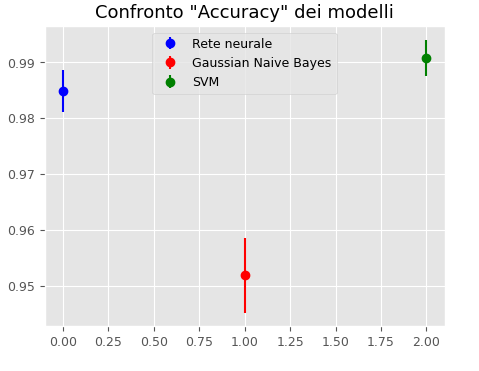
\includegraphics[width=\textwidth]{img/ris/accuracy_inter_corr.png}
        \caption{Accuracy}
        \label{fig:acc}
    \end{subfigure}
    \hfill
    \begin{subfigure}[b]{0.4\textwidth}
        \centering
        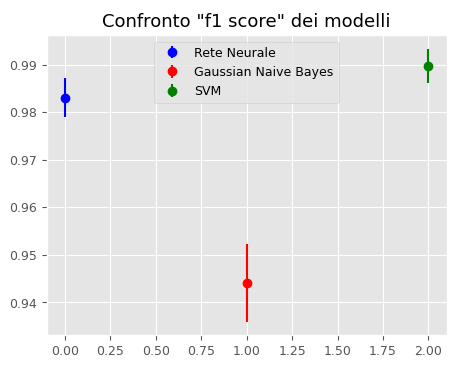
\includegraphics[width=\textwidth]{img/ris/fscore_inter_corr.png}
        \caption{F1 score}
        \label{fig:f1}
    \end{subfigure}
    \hfill
    \begin{subfigure}[b]{0.4\textwidth}
        \centering
        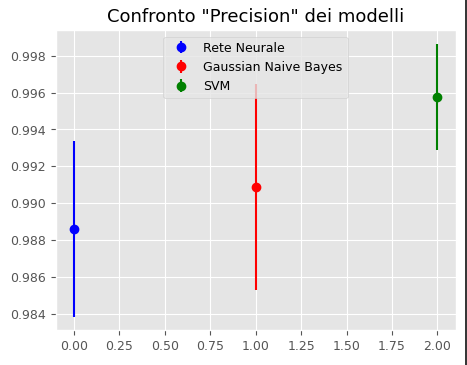
\includegraphics[width=\textwidth]{img/ris/precision_inter_corr.png}
        \caption{Precision}
        \label{fig:precision}
    \end{subfigure}
    \hfill
    \begin{subfigure}[b]{0.4\textwidth}
        \centering
        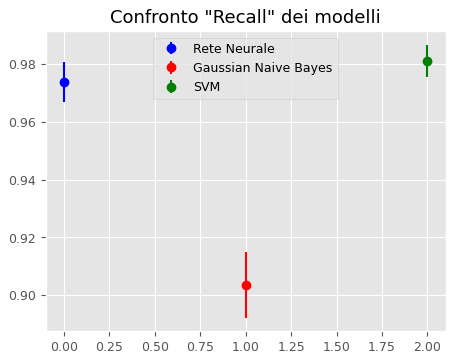
\includegraphics[width=\textwidth]{img/ris/recall_inter_corr.png}
        \caption{Recall}
        \label{fig:recall}
    \end{subfigure}
    \caption{Intervalli di confidenza ottenuti dai modelli addestrati con e senza PCA}
    \label{fig:img_intervalli_confidenza_corr}
\end{figure}

Dagli intervalli di confidenza si nota immediatamente che Gaussian Naive Bayes è
il peggiore rispetto agli altri modelli secondo le metriche di Accuracy, Recall
e F1-score, non solo in termini di media degli intervalli, ma anche in termini
di varianza delle metriche. Questo significa che tra tutti i modelli allenati
sulla versione \texttt{dataset\_corr} \texttt{dataset\_corr\_std}, i migliori
sono quelli che manipolano i dati geometricamente, più precisamente si hanno
risultati migliori del circa $4\%-8\%$ sulle metriche di Accuracy, Recall e
F1-score. Al contrario la Precision di Gaussian Naive Bayes risulta più
confrontabile con gli altri modelli, ma suggerisce solo che si hanno pochi
errori sulla classe positiva come anche dimostrato dalla matrice di confusione
di tale modello. Il problema è che le altre metriche specificano più errori
sulla classe negativa che nel dominio in questione non è una caratteristica
accettabile, dal momento che l'obiettivo dovrebbe essere quello di ridurre il
più possibile i falsi negativi, massimizzando la Recall, ma massimizzando il più
possibile la precision. Con tutte queste osservazioni il modello migliore è SVM
dal momento che in generare ha degli ottimi risultati sia in termini di
correttezza nella classificazione, sia in termini di minimizzazione dei falsi
negativi, mantenendo un ridotto errore dei falsi positivi.
\section{Risultati dei modelli allenati su \texttt{dataset\_pca} e
  \texttt{dataset\_pca\_std}} \label{sec:risultati_pca}
Un ragionamento analogo a quello svolto nella sezione \ref{sec:risultati_corr}
può essere applicato ai modelli addestrati sul dataset le cui feature sono state
selezionate attraverso Principal Component Analysis (PCA).

Per questa analisi, il primo passo consisteva nel calcolare le matrici di
confusione per ciascun modello. Le matrici di confusione sono state generare sia
per il dataset \texttt{dataset\_pca} che per il dataset \texttt{dataset\_pca\_std},
e i risultati sono illustrati nella figura \ref{fig:matrice_di_confusione_per_pca}.
\begin{figure}[!ht]
    \centering
    \begin{subfigure}{0.45\textwidth}
        \centering
        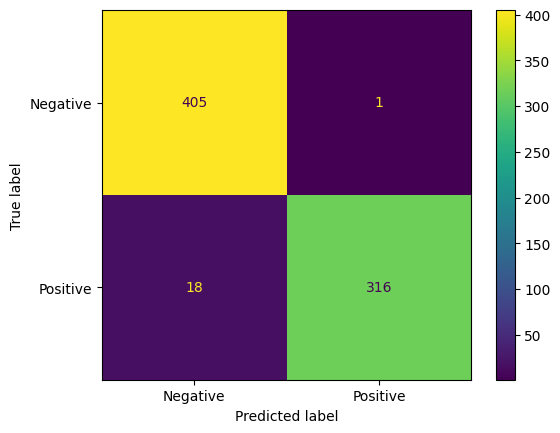
\includegraphics[width=\textwidth]{img/svm/matrice_confusione_pca.png}
        \caption{Support Vector Machine}
        \label{fig:matrice_di_confusione_per_SVM_pca}
    \end{subfigure}
    \hfill
    \begin{subfigure}{.45\textwidth}
        \centering
        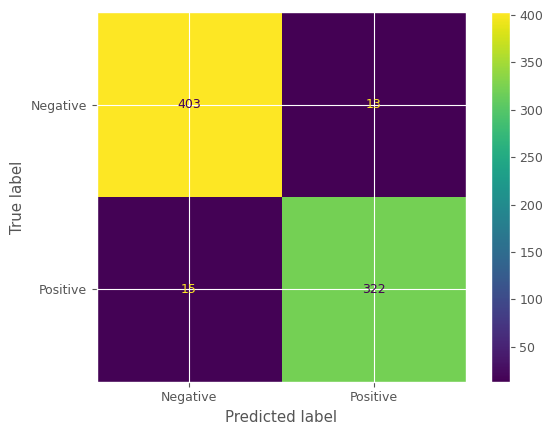
\includegraphics[width=\textwidth]{img/gnb/confusion_matrix_pca.png}
        \caption{Gaussian Naive Bayes}
        \label{fig:matrice_di_confusione_per_GNB_pca}
    \end{subfigure}
    \hfill
    \begin{subfigure}{.45\textwidth}
        \centering
        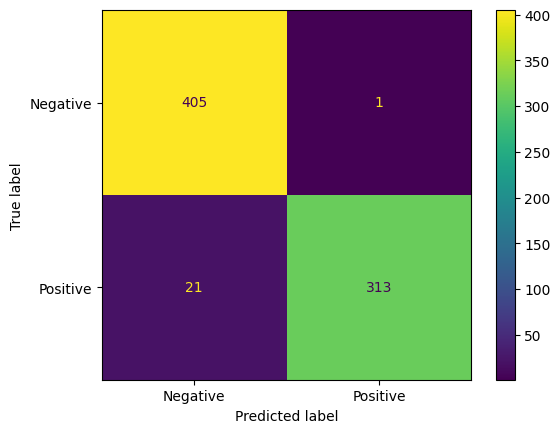
\includegraphics[width=\textwidth]{img/rete/matrice_confusione_PCA.png}
        \caption{Rete neurale}
        \label{fig:matrice_di_confusione_per_NN_pca}
    \end{subfigure}
    \caption{Matrici di confusione per i modelli addestrati su \texttt{dataset\_pca} e \texttt{dataset\_pca\_std}}
    \label{fig:matrice_di_confusione_per_pca}
\end{figure}

Dalle matrici di confusione si evidenzia come Gaussian Naive Bayes continua ad
essere il modello che presenta un numero più elevato di errori rispetto agli
altri due, in ogni caso si uniforma agli altri a livello di falsi negativi,
aumentando però il numero di falsi positivi. Per completezza sono state ricavate
dalle matrici di confusione le metriche di valutazione dei vari modelli e i
valori ottenuti sono stati riportati nella tabella \ref{tab:risultati_pca}.
\begin{table}[!ht]
    \centering
    \begin{tabular}{@{}clllll@{}}
        \toprule
        \rowcolor[HTML]{EFEFEF}
        \textbf{Modello}                                      & \textbf{Accuracy}            & \textbf{Precision}           & \textbf{Recall}              & \textbf{F1-score}            & \textbf{Tempo}              \\ \midrule
        \cellcolor[HTML]{EFEFEF}\textbf{SVM}                  & \multicolumn{1}{c}{97.43 \%} & \multicolumn{1}{c}{100 \%}   & \multicolumn{1}{c}{94.31 \%} & \multicolumn{1}{c}{97.07 \%} & \multicolumn{1}{c}{0.196 s} \\
        \cellcolor[HTML]{EFEFEF}\textbf{Gaussian Naive Bayes} & \multicolumn{1}{c}{96 \%}    & \multicolumn{1}{c}{96 \%}    & \multicolumn{1}{c}{96 \%}    & \multicolumn{1}{c}{96 \%}    & \multicolumn{1}{c}{0.006 s} \\
        \cellcolor[HTML]{EFEFEF}\textbf{Rete neurale}         & \multicolumn{1}{c}{98.27 \%} & \multicolumn{1}{c}{97.92 \%} & \multicolumn{1}{c}{98.21 \%} & \multicolumn{1}{c}{98.07 \%} & \multicolumn{1}{c}{3.326 s} \\ \bottomrule
    \end{tabular}
    \caption{Risultati ottenuti dal modello addestrato}
    \label{tab:risultati_pca}
\end{table}

I risultati ottenuti rivelano prestazioni molto simili a quelle osservate nel
dataset le cui feature sono state selezionate manualmente. Questo ci suggerisce
che l'applicazione di PCA potrebbe essere un operazione superflua. Questa idea
deve essere ulteriormente verificata attraverso l'analisi delle curve ROC e
il processo di valutazione attraverso la cross-validation.

In aggiunta all'analisi sulle metriche, è stato condotto un confronto tra i
modelli mediante l'utilizzo delle curve ROC, le quali sono presentate nella
figura \ref{fig:roc_curve_pca}.
\begin{figure}[!ht]
    \centering
    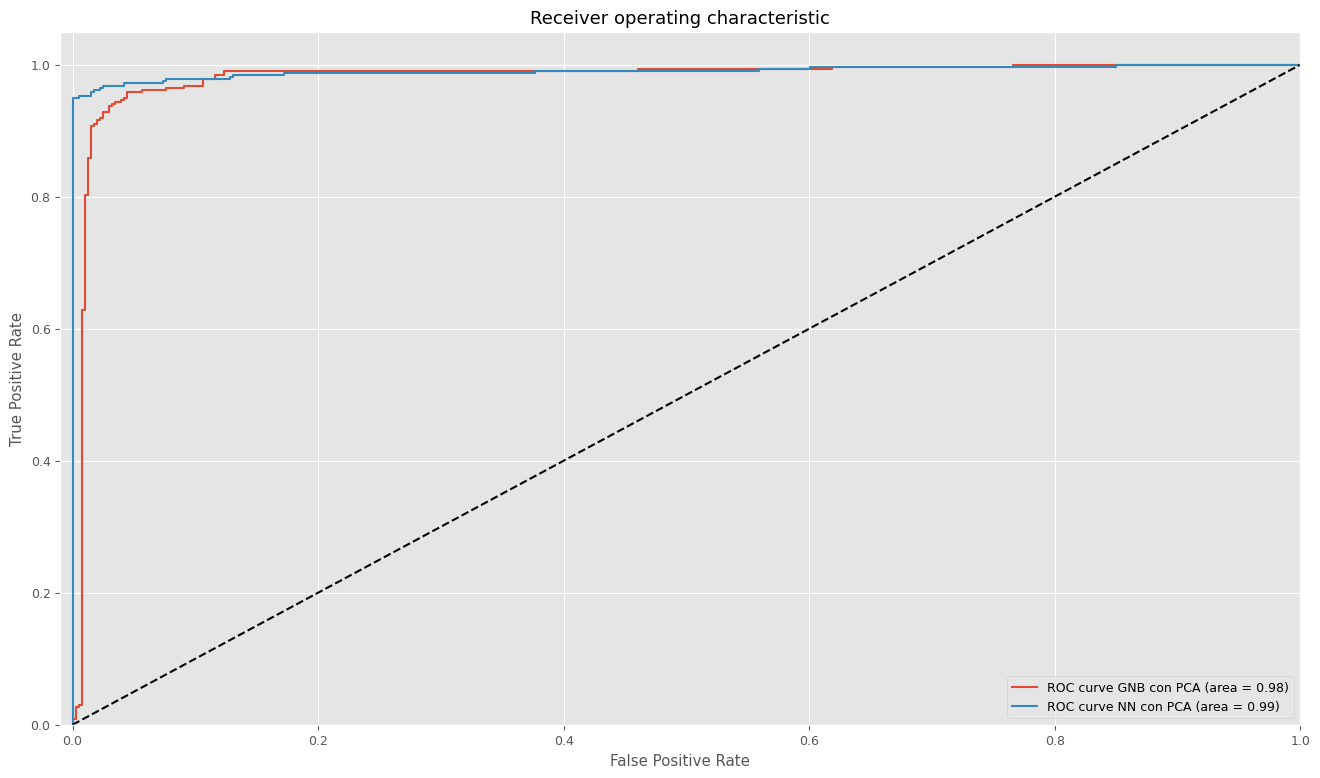
\includegraphics[width=\textwidth]{img/ris/roc_curve_pca.png}
    \caption{Curve ROC per i modelli addestrati su \texttt{dataset\_pca} e \texttt{dataset\_pca\_std}}
    \label{fig:roc_curve_pca}
\end{figure}

Nelle curve ROC create con i modelli addestrati sul dataset estratto con PCA, si
può notare una maggiore distanza tra le curve della rete neurale e SVM rispetto
a quella del Gaussian Naive Bayes. Questo si nota principalmente nella parte
sinistra del grafico, dove si ha un tasso di falsi positivi molto basso.

In casi come questo, dove le curve ROC sono molto simili, è possibile confrontare
i modelli in termini di AUC. L'area sottesa alla curva ROC per la rete neurale e
della SVM sono pari a $0.99$, mentre per il Gaussian Naive Bayes è pari a $0.98$.
Questi valori suggeriscono che i modelli basati sulla manipolazione geometrica
siano leggermente superiori a Gaussian Naive Bayes in termini di capacità di
discriminazione tra le due classi.

Questo studio suggerisce che l'applicazione di PCA non ha portato a miglioramenti
significativi nelle performance dei modelli.
\newpage
Per concludere, è stato condotto uno studio di robustezza dei modelli tramite
la tecnica della $10$-fold stratified cross-validation. I risultati ottenuti
sono stati riportati in figura \ref{fig:intervalli_confidenza_pca} e nella
tabella \ref{tab:intervalli_confidenza_pca}.
\begin{table}[!ht]
    \begin{subtable}[h]{1\textwidth}
        \centering
        \begin{tabular}{@{}cllll@{}}
            \toprule
            \rowcolor[HTML]{EFEFEF}
            \textbf{Modello}                                      & \textbf{Accuratezza}         & \textbf{Precisione}          & \textbf{Richiamo}            & \textbf{F1 score}            \\ \midrule
            \cellcolor[HTML]{EFEFEF}\textbf{SVM}                  & \multicolumn{1}{c}{99.05 \%} & \multicolumn{1}{c}{99.57 \%} & \multicolumn{1}{c}{98.32 \%} & \multicolumn{1}{c}{98.94 \%} \\
            \cellcolor[HTML]{EFEFEF}\textbf{Gaussian Naive Bayes} & \multicolumn{1}{c}{96 \%}    & \multicolumn{1}{c}{96 \%}    & \multicolumn{1}{c}{96 \%}    & \multicolumn{1}{c}{96 \%}    \\
            \cellcolor[HTML]{EFEFEF}\textbf{Rete neurale}         & \multicolumn{1}{c}{98.35 \%} & \multicolumn{1}{c}{98.05 \%} & \multicolumn{1}{c}{98.27 \%} & \multicolumn{1}{c}{98.15 \%} \\ \bottomrule
        \end{tabular}
        \caption{Valore medio delle metriche ottenute dalla cross validation}
        \label{tab:risultati_cross_val_pca}
    \end{subtable}
    \hfill
    \begin{subtable}[h]{1\textwidth}
        \centering
        \begin{tabular}{@{}cllll@{}}
            \toprule
            \rowcolor[HTML]{EFEFEF}
            \textbf{Modello}                                      & \textbf{Accuratezza} & \textbf{Precisione} & \textbf{Richiamo}  & \textbf{F1 score}  \\ \midrule
            \cellcolor[HTML]{EFEFEF}\textbf{SVM}                  & [98.75\%, 99.35\%]   & [99.34\%, 99.81\%]  & [97.65\%, 98.99\%] & [98.60\%, 99.27\%] \\
            \cellcolor[HTML]{EFEFEF}\textbf{Gaussian Naive Bayes} & [94.73\%, 95.85\%]   & [98.65\%, 99.53\%]  & [89.14\%, 91.70\%] & [93.85\%, 95.22\%] \\
            \cellcolor[HTML]{EFEFEF}\textbf{Rete neurale}         & [97.97\%, 98.72\%]   & [97.51\%, 98.58\%]  & [97.62\%, 98.93\%] & [97.73\%, 98.58\%] \\ \bottomrule
        \end{tabular}
        \caption{Intervalli di confidenza delle metriche ottenute dalla cross validation}
        \label{tab:intervalli_confidenza_pca}
    \end{subtable}
    \caption{Risultati ottenuti dalla cross validation}
    \label{tab:media_intervalli_confidenza_pca}
\end{table}

Analizzando i risultati della cross-validation, si può notare che i modelli
basati sulla manipolazione geometrica dei dati continuano a mostrare performance
superiori rispetto a Gaussian Naive Bayes. In particolare, SVM è il modello che
mostra le performance migliori si in termini di media delle metriche, sia in
termini di varianza delle stesse. Questo suggerisce che SVM è il modello più
robusto tra i tre.

A differenza di quanto osservato nel dataset le cui feature sono state selezionate
manualmente, in questo caso l'applicazione di PCA ha portato a degli intervalli
di confidenza leggermente più piccoli per quanto riguarda la rete neurale, 
suggerendo che l'applicazione di PCA potrebbe aver portato a una maggiore
robustezza del modello.
Per quanto riguarda Gaussian Naive Bayes si hanno valori medi delle metriche
minori rispetto agli altri modelli, e con intervalli di confidenza più ampi
nella maggior parte delle metriche, suggerendo che questo modello è il meno
robusto tra i tre.
\begin{figure}[!ht]
    \centering
    \begin{subfigure}[b]{0.4\textwidth}
        \centering
        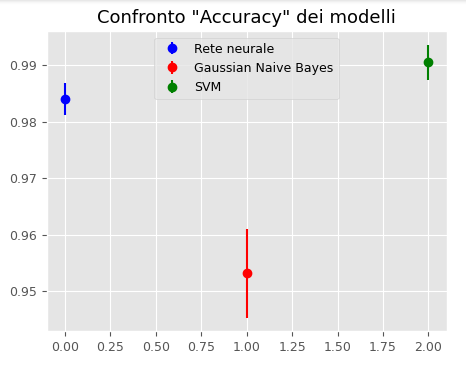
\includegraphics[width=\textwidth]{img/ris/accuracy_inter_pca.png}
        \caption{Accuracy}
        \label{fig:acc_pca}
    \end{subfigure}
    \hfill
    \begin{subfigure}[b]{0.4\textwidth}
        \centering
        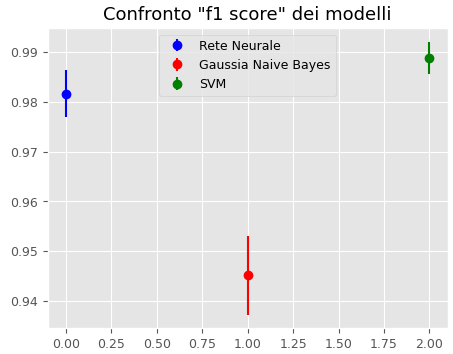
\includegraphics[width=\textwidth]{img/ris/fscore_inter_pca.png}
        \caption{F1 score}
        \label{fig:f1_pca}
    \end{subfigure}
    \hfill
    \begin{subfigure}[b]{0.4\textwidth}
        \centering
        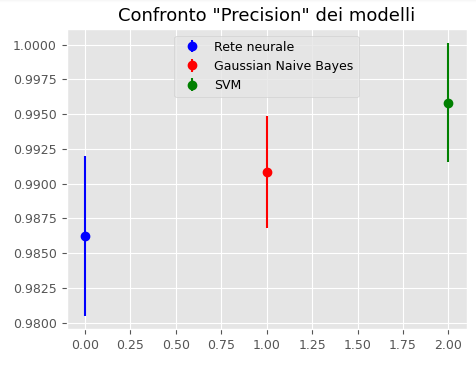
\includegraphics[width=\textwidth]{img/ris/precision_inter_pca.png}
        \caption{Precision}
        \label{fig:precision_pca}
    \end{subfigure}
    \hfill
    \begin{subfigure}[b]{0.4\textwidth}
        \centering
        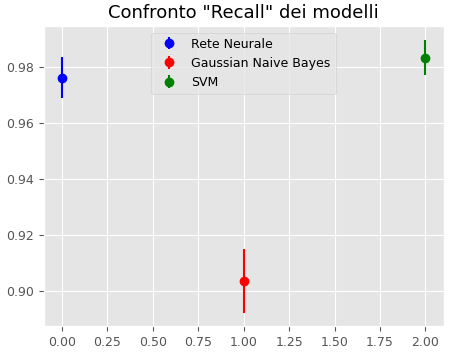
\includegraphics[width=\textwidth]{img/ris/recall_inter_pca.png}
        \caption{Recall}
        \label{fig:recall_pca}
    \end{subfigure}
    \caption{Intervalli di confidenza ottenuti dai modelli addestrati con e senza PCA}
    \label{fig:intervalli_confidenza_pca}
\end{figure}